% Provenance (never printed): see sources/outline_sources.md (Year 1:
% astronomy of position, spherical trigonometry, time scales, insolation).
% Spherical trigonometry is absent from the mathematics series: this chapter
% owns it. Curves computed in figdata/bachelor-1/{sun_paths, day_length,
% celestial_sphere, spherical_triangle}.py (shared model _solar.py); numbers
% of the exercises and problem in the Book 3 scratch calculator ch01.py.
\chapter{Spherical Astronomy}\label{ch:b1:spherical-astronomy}

On a clear night far from any town, a long-exposure camera pointed at the
sky records the stars as arcs of circles, all centred on one point that does
not move. A star that rose in the east at nine o'clock tonight will rise at
about five to nine tomorrow, and a little earlier every night after that. The
Sun at noon stands higher in June than in December, and in the far north it
does not set at all in midsummer. All of this is the rotation of the Earth
and its orbit round the Sun, seen from the ground. To describe it, the
astronomer and the geoscientist need coordinates on a sphere, the
trigonometry of triangles drawn on a sphere, and clocks that keep step with
the stars or with the Sun. This chapter builds these tools. They return in
plate kinematics (\cref{ch:b1:plate-kinematics}), where plates turn on the
sphere, and in the climate chapters (\cref{ch:b1:radiation-heat-transport}),
where the sunlight a \omterm{def:b1:spherical-astronomy:geographic}{latitude} receives drives the winds and the currents.

\begin{recall}
The Earth turns on its axis once a day and goes round the Sun once a year on
an orbit that is very nearly a circle; its axis is tilted with respect to the
orbit, which makes the seasons (the physics books, grades 6 and 12; Kepler's
laws are recalled from the physics books' Year 1 volume). A point on the Earth
is located by its \omterm{def:b1:spherical-astronomy:geographic}{latitude} and \omterm{def:b1:spherical-astronomy:geographic}{longitude} (Book 1, grade 6). A vector of length
one is fixed by two angles, as in spherical coordinates; the dot product of
two unit vectors is the cosine of the angle between them, and the triple
product $\vec u\cdot(\vec v\times\vec w)$ is unchanged by a cyclic
permutation of the three vectors.
\end{recall}

\section{Triangles on a sphere}

\begin{definition}[Great circle, spherical triangle]\label{def:b1:spherical-astronomy:spherical-triangle}
A \emph{great circle}\index{great circle} of a sphere is its intersection
with a plane through its centre; any other plane section is a \emph{small
circle}\index{small circle}. Through two points that are not diametrically
opposite passes exactly one great circle, and the shorter of its two arcs is
the shortest path on the sphere between the points. A \emph{spherical
triangle}\index{spherical triangle} is the figure formed by three points of
the sphere, its vertices $A$, $B$, $C$, joined by arcs of great circles of
less than \ang{180}. Its sides $a$, $b$, $c$ (opposite $A$, $B$, $C$) are
measured by the angles they subtend at the centre; its angles $A$, $B$, $C$
are the angles between the planes of the sides that meet at each vertex.
\end{definition}

On the sphere of radius $R$, a side of $a$ radians has the length $Ra$. Every
side and every angle lies between $0$ and $\pi$.

\begin{omfigure}
\begin{tikzpicture}
\begin{axis}[x=1cm, y=1cm, hide axis, xmin=-2.7, xmax=2.7, ymin=-2.6, ymax=2.6, clip=false]
\draw[black, line width=0.6pt] (axis cs:0,0) circle (2.4cm);
\addplot[black!45, densely dashed, line width=0.4pt] coordinates {(0,0) (-0.078358,1.7847)};
\addplot[black!45, densely dashed, line width=0.4pt] coordinates {(0,0) (-1.5903,-0.2902)};
\addplot[black!45, densely dashed, line width=0.4pt] coordinates {(0,0) (1.4453,-0.16381)};
\addplot[omDef, line width=1.1pt] table {figdata/out/bachelor-1-spherical_triangle-ab.dat};
\addplot[omDef, line width=1.1pt] table {figdata/out/bachelor-1-spherical_triangle-bc.dat};
\addplot[omDef, line width=1.1pt] table {figdata/out/bachelor-1-spherical_triangle-ca.dat};
\addplot[omThm, line width=0.8pt] table {figdata/out/bachelor-1-spherical_triangle-angA.dat};
\addplot[only marks, mark=*, mark size=1.4pt] table[x=x, y=y] {figdata/out/bachelor-1-spherical_triangle-verts.dat};
\fill (axis cs:0,0) circle (1.2pt);
\begin{scope}[font=\small]
  \node[above] at (axis cs:-0.078358,1.7847) {$A$};
  \node[left] at (axis cs:-1.5903,-0.2902) {$B$};
  \node[right] at (axis cs:1.4453,-0.16381) {$C$};
  \node[above left] at (axis cs:0,0) {$O$};
  \node[omThm] at (axis cs:0.24,1.36) {$A$};
  \node[omDef] at (axis cs:0.0,-0.52) {$a$};
  \node[omDef] at (axis cs:0.95,0.95) {$b$};
  \node[omDef] at (axis cs:-1.05,0.95) {$c$};
\end{scope}
\end{axis}
\end{tikzpicture}

{\small A \omterm{def:b1:spherical-astronomy:spherical-triangle}{spherical triangle} $ABC$ on a sphere of centre $O$. The sides $a$,
$b$, $c$ are arcs of \omterm{def:b1:spherical-astronomy:spherical-triangle}{great circles}, measured by the angles $BOC$, $COA$,
$AOB$; the angle $A$ (red) is the angle between the two sides that meet at
$A$. The triangle drawn has $a = \ang{78.6}$, $b = \ang{62.6}$,
$c = \ang{64.8}$ and angles of \ang{89.9}, \ang{64.9} and \ang{67.4}, which
add up to more than \ang{180}.}
\end{omfigure}

\begin{theorem}[The cosine rule]\label{thm:b1:spherical-astronomy:cosine-rule}
In a \omterm{def:b1:spherical-astronomy:spherical-triangle}{spherical triangle},
\[
  \cos a = \cos b\cos c + \sin b\sin c\cos A .
\]
\end{theorem}

\begin{proof}
Work on the unit sphere and choose axes with $A$ at the pole:
$\vec A = (0, 0, 1)$, and the plane $xz$ containing $B$:
$\vec B = (\sin c, 0, \cos c)$, since $B$ is at the angular distance $c$ from
$A$. The point $C$ is at the angular distance $b$ from $A$, on a \omterm{def:b1:spherical-astronomy:spherical-triangle}{great circle}
through $A$ making the angle $A$ with the plane $xz$:
$\vec C = (\sin b\cos A, \sin b\sin A, \cos b)$. The side $a$ is the angle
between $\vec B$ and $\vec C$, so
\[
  \cos a = \vec B\cdot\vec C = \sin c\sin b\cos A + \cos c\cos b. \qedhere
\]
\end{proof}

\begin{theorem}[The sine rule]\label{thm:b1:spherical-astronomy:sine-rule}
In a \omterm{def:b1:spherical-astronomy:spherical-triangle}{spherical triangle},
\[
  \frac{\sin A}{\sin a} = \frac{\sin B}{\sin b} = \frac{\sin C}{\sin c}.
\]
\end{theorem}

\begin{proof}
With the vectors of the previous proof,
$\vec B \times \vec C = (-\cos c\sin b\sin A,\ \cos c\sin b\cos A - \sin c\cos b,\
\sin c\sin b\sin A)$, so the triple product is
$\vec A\cdot(\vec B\times\vec C) = \sin b\sin c\sin A$. The triple product is
unchanged when $A$, $B$, $C$ are permuted cyclically; placing $B$, then $C$,
at the pole gives in the same way $\sin c\sin a\sin B$ and $\sin a\sin b\sin
C$. The three expressions are equal; dividing by $\sin a\sin b\sin c$ gives
the rule.
\end{proof}

When the sides are small compared with the radius, $\cos a \approx 1 -
a^2/2$ and $\sin a \approx a$, and the two rules become the cosine and sine
rules of plane triangles: on a small enough patch the sphere is flat. On a
large triangle they do not: the angles of a \omterm{def:b1:spherical-astronomy:spherical-triangle}{spherical triangle} add up to more
than \ang{180} (\cref{exo:b1:spherical-astronomy:12}).

\begin{method}[Distance and heading on the sphere]\label{met:b1:spherical-astronomy:great-circle}
To find the shortest distance between two places of \omterm{def:b1:spherical-astronomy:geographic}{latitudes} $\varphi_1$,
$\varphi_2$ and \omterm{def:b1:spherical-astronomy:geographic}{longitudes} $\lambda_1$, $\lambda_2$, and the direction in
which to set off:
\begin{enumerate}
  \item form the triangle with vertices the North Pole $P$ and the two
        places; its sides from the pole are the colatitudes $\ang{90} -
        \varphi_1$ and $\ang{90} - \varphi_2$, and its angle at the pole is
        the difference of \omterm{def:b1:spherical-astronomy:geographic}{longitude} $\Delta\lambda$;
  \item the cosine rule gives the angular distance $\Delta$:
        $\cos\Delta = \sin\varphi_1\sin\varphi_2 +
        \cos\varphi_1\cos\varphi_2\cos\Delta\lambda$; the distance is
        $R\Delta$ ($\Delta$ in radians);
  \item the initial heading is the angle of the triangle at the first place,
        from the cosine rule applied to the side opposite it,
        $\sin\varphi_2 = \sin\varphi_1\cos\Delta + \cos\varphi_1\sin\Delta\cos
        \mathrm{Az}$, and is measured from north toward the second place.
\end{enumerate}
The heading changes along the \omterm{def:b1:spherical-astronomy:spherical-triangle}{great circle} (except along a meridian or the
equator): a ship or aircraft that keeps the same compass heading follows
another, longer curve.
\end{method}

\section{Coordinates on the sphere}

\begin{definition}[Latitude and longitude]\label{def:b1:spherical-astronomy:geographic}
Let the Earth be a sphere turning about its polar axis. The
\emph{latitude}\index{latitude} $\varphi$ of a point is the angle between
the equatorial plane and the radius through the point, from \ang{-90}
(South Pole) to \ang{+90} (North Pole); its \emph{longitude}\index{longitude}
$\lambda$ is the angle, measured in the equatorial plane, between the
meridian half-plane of the point and that of a reference meridian, the one
through Greenwich, counted positive to the east, from \ang{-180} to
\ang{180}.
\end{definition}

The Earth is in fact slightly flattened; the \omterm{def:b1:spherical-astronomy:geographic}{latitude} used for maps and for
the sky is the angle between the local vertical and the equatorial plane,
which differs from the geocentric angle by at most \ang{0.2}
(\cref{ch:b1:isostasy-gravity}). Lines of equal \omterm{def:b1:spherical-astronomy:geographic}{latitude}, the parallels, are
\omterm{def:b1:spherical-astronomy:spherical-triangle}{small circles}; the meridians are halves of \omterm{def:b1:spherical-astronomy:spherical-triangle}{great circles}.

\begin{definition}[The celestial sphere]\label{def:b1:spherical-astronomy:celestial-sphere}
The \emph{celestial sphere}\index{celestial sphere} is an imaginary sphere
centred on the observer, on which every star is placed in its direction; only
directions matter, not distances. The extensions of the Earth's axis meet it
at the north and south \emph{celestial poles}\index{celestial pole}; the
plane of the Earth's equator cuts it along the \emph{celestial
equator}\index{celestial equator}. The \emph{zenith}\index{zenith} is the
point straight overhead, along the local vertical; the horizon is the \omterm{def:b1:spherical-astronomy:spherical-triangle}{great
circle} $\ang{90}$ from it. The \emph{local meridian}\index{local meridian} is
the \omterm{def:b1:spherical-astronomy:spherical-triangle}{great circle} through the zenith and the celestial poles; it meets the
horizon at the north and south points.
\end{definition}

As the Earth turns from west to east, the \omterm{def:b1:spherical-astronomy:celestial-sphere}{celestial sphere} seems to turn the
other way, from east to west, about the axis of the \omterm{def:b1:spherical-astronomy:celestial-sphere}{celestial poles}, once in
a little less than a day. The stars keep their relative places: they are so
far away that a year's journey round the Sun changes their directions by
less than a second of arc (\cref{ch:b1:observing-the-sky}).

\begin{definition}[Horizontal coordinates]\label{def:b1:spherical-astronomy:horizontal}
The \emph{altitude}\index{altitude (of a star)} $h$ of a star is its angle
above the horizon, from \ang{-90} to \ang{90}; its \omterm{def:b1:spherical-astronomy:celestial-sphere}{zenith} distance is
$z = \ang{90} - h$. Its \emph{azimuth}\index{azimuth} $\mathrm{A}$ is the
angle, along the horizon, from the north point to the foot of the star's
vertical circle, counted from \ang{0} to \ang{360} through the east.
\end{definition}

Horizontal coordinates are those of the observer: they change with place and
time. The coordinates of the sky itself are carried along by its rotation.

\begin{definition}[Equatorial coordinates]\label{def:b1:spherical-astronomy:equatorial}
The \emph{declination}\index{declination (celestial)} $\delta$ of a star is
its angle from the \omterm{def:b1:spherical-astronomy:celestial-sphere}{celestial equator}, positive to the north, from \ang{-90}
to \ang{90}. The \omterm{def:b1:spherical-astronomy:spherical-triangle}{great circle} through the star and the \omterm{def:b1:spherical-astronomy:celestial-sphere}{celestial poles} is its
hour circle. The \emph{hour angle}\index{hour angle} $H$ of the star is the
angle at the \omterm{def:b1:spherical-astronomy:celestial-sphere}{celestial pole} between the \omterm{def:b1:spherical-astronomy:celestial-sphere}{local meridian} and the star's hour
circle, counted westward, in hours of \ang{15}. The \emph{right
ascension}\index{right ascension} $\alpha$ is the angle along the \omterm{def:b1:spherical-astronomy:celestial-sphere}{celestial
equator} from a fixed point of the sky, the \omterm{def:b1:spherical-astronomy:ecliptic}{vernal equinox point}
(\cref{def:b1:spherical-astronomy:ecliptic}), to the star's hour circle,
counted eastward, also in hours.
\end{definition}

\omterm{def:b1:spherical-astronomy:equatorial}{Declination} and \omterm{def:b1:spherical-astronomy:equatorial}{right ascension} are fixed on the sky, like \omterm{def:b1:spherical-astronomy:geographic}{latitude} and
\omterm{def:b1:spherical-astronomy:geographic}{longitude} on the Earth: catalogues list them. The word \omterm{def:b1:spherical-astronomy:equatorial}{declination} is used
here in this astronomical sense only; the angle between geographic north and
the north of a compass is always called the magnetic declination
(\cref{ch:b1:field-lab-methods-1}).

\begin{proposition}[From equatorial to horizontal coordinates]\label{prop:b1:spherical-astronomy:transform}
At \omterm{def:b1:spherical-astronomy:geographic}{latitude} $\varphi$, a star of \omterm{def:b1:spherical-astronomy:equatorial}{declination} $\delta$ and \omterm{def:b1:spherical-astronomy:equatorial}{hour angle} $H$ has
the \omterm{def:b1:spherical-astronomy:horizontal}{altitude} and \omterm{def:b1:spherical-astronomy:horizontal}{azimuth} given by
\[
  \sin h = \sin\varphi\sin\delta + \cos\varphi\cos\delta\cos H,
  \qquad
  \cos\mathrm{A} = \frac{\sin\delta - \sin\varphi\sin h}{\cos\varphi\cos h},
\]
with $\mathrm{A}$ between \ang{0} and \ang{180} when the star is east of the
meridian ($\sin H < 0$) and $\mathrm{A} = \ang{360} - \arccos(\dots)$ when it
is west. In particular the \omterm{def:b1:spherical-astronomy:horizontal}{altitude} of the north \omterm{def:b1:spherical-astronomy:celestial-sphere}{celestial pole} equals the
\omterm{def:b1:spherical-astronomy:geographic}{latitude}.
\end{proposition}

\begin{proof}
Consider the triangle formed by the north \omterm{def:b1:spherical-astronomy:celestial-sphere}{celestial pole} $P$, the \omterm{def:b1:spherical-astronomy:celestial-sphere}{zenith} $Z$
and the star $X$ (the astronomical, or position, triangle). The local
vertical makes the angle $\varphi$ with the equatorial plane, so $PZ =
\ang{90} - \varphi$; $PX = \ang{90} - \delta$; $ZX = \ang{90} - h$. The angle
at $P$ is the \omterm{def:b1:spherical-astronomy:equatorial}{hour angle} $H$; the angle at $Z$ is the \omterm{def:b1:spherical-astronomy:horizontal}{azimuth} of the star
measured from north (east or west of the meridian). The cosine rule for the
side $ZX$, opposite $P$, gives
$\cos(\ang{90} - h) = \cos(\ang{90} - \varphi)\cos(\ang{90} - \delta) +
\sin(\ang{90} - \varphi)\sin(\ang{90} - \delta)\cos H$, the first formula.
The cosine rule for the side $PX$, opposite $Z$, gives
$\sin\delta = \sin\varphi\sin h + \cos\varphi\cos h\cos\mathrm{A}$, the
second. For the pole, $\delta = \ang{90}$ and the first formula reads
$\sin h = \sin\varphi$.
\end{proof}

\begin{omfigure}
\begin{tikzpicture}
\pic (cs) at (0,0) {celestialsphere=45};
\begin{axis}[x=1cm, y=1cm, hide axis, anchor=origin, at={(0,0)}, xmin=-2.6, xmax=2.6, ymin=-2.4, ymax=2.5, clip=false]
\addplot[omField, line width=1.1pt] table[x=x, y=y] {figdata/out/bachelor-1-celestial_sphere-vertical.dat};
\addplot[black!80, line width=0.9pt, densely dash dot] table[x=x, y=y] {figdata/out/bachelor-1-celestial_sphere-hourcircle.dat};
\addplot[only marks, mark=star, mark size=3pt, mark options={line width=0.8pt}] table[x=x, y=y] {figdata/out/bachelor-1-celestial_sphere-star.dat};
\end{axis}
\begin{scope}[font=\footnotesize]
  \node[above] at (cs-Z) {$Z$};
  \node[above left] at (cs-NCP) {$P$};
  \node[left] at (cs-N) {N};
  \node[right] at (cs-S) {S};
  \node[below] at (cs-W) {W};
  \node[below, fill=white, fill opacity=0.8, text opacity=1, inner sep=1pt] at (cs-E) {E};
  \node[above right] at (0.2262,0.94) {$X$};
  \node[omField] at (0.55,0.2) {$h$};
  \node[omDef, right] at (2.0,-1.25) {equator};
  \node[left] at (-2.0,-0.3) {horizon};
  \node at (-1.35,0.62) {$\varphi$};
\end{scope}
\draw[black!60, line width=0.4pt] (-1.05,0) arc[start angle=180, end angle=137, radius=1.05cm];
\end{tikzpicture}

{\small The sky at \omterm{def:b1:spherical-astronomy:geographic}{latitude} \ang{45} N, seen from the west, north on the
left. The north \omterm{def:b1:spherical-astronomy:celestial-sphere}{celestial pole} $P$ stands at an \omterm{def:b1:spherical-astronomy:horizontal}{altitude} equal to the
\omterm{def:b1:spherical-astronomy:geographic}{latitude} above the north point (red: the axis of the \omterm{def:b1:spherical-astronomy:celestial-sphere}{celestial poles}); the
\omterm{def:b1:spherical-astronomy:celestial-sphere}{celestial equator} (blue) crosses the
horizon at the east and west points. A star $X$ of \omterm{def:b1:spherical-astronomy:equatorial}{declination} \ang{25},
three hours twenty minutes after its passage across the meridian (\omterm{def:b1:spherical-astronomy:equatorial}{hour angle}
\ang{50}), is at the \omterm{def:b1:spherical-astronomy:horizontal}{altitude} $h = \ang{45.3}$ (green: its vertical circle,
from the \omterm{def:b1:spherical-astronomy:celestial-sphere}{zenith} $Z$ to the horizon) and the \omterm{def:b1:spherical-astronomy:horizontal}{azimuth} \ang{261}; its hour
circle (dash-dotted) runs from the pole through the star to the equator.
Computed with \cref{prop:b1:spherical-astronomy:transform}.}
\end{omfigure}

\begin{proposition}[Culmination and circumpolar stars]\label{prop:b1:spherical-astronomy:culmination}
At \omterm{def:b1:spherical-astronomy:geographic}{latitude} $\varphi$, a star of \omterm{def:b1:spherical-astronomy:equatorial}{declination} $\delta$ crosses the meridian
($H = 0$) at the \omterm{def:b1:spherical-astronomy:horizontal}{altitude} $\ang{90} - |\varphi - \delta|$, south of the \omterm{def:b1:spherical-astronomy:celestial-sphere}{zenith}
if $\delta < \varphi$, north of it if $\delta > \varphi$. In the northern
hemisphere ($\varphi > 0$) it never sets if $\delta > \ang{90} - \varphi$ and
never rises if $\delta < -(\ang{90} - \varphi)$.
\end{proposition}

\begin{proof}
For $H = 0$, $\sin h = \sin\varphi\sin\delta + \cos\varphi\cos\delta =
\cos(\varphi - \delta)$, so $h = \ang{90} - |\varphi - \delta|$. The lowest
\omterm{def:b1:spherical-astronomy:horizontal}{altitude}, at $H = \ang{180}$, satisfies $\sin h = -\cos(\varphi + \delta)$;
it is positive when $\varphi + \delta > \ang{90}$. The star stays below the
horizon when even its highest \omterm{def:b1:spherical-astronomy:horizontal}{altitude} is negative,
$|\varphi - \delta| > \ang{90}$.
\end{proof}

\begin{definition}[Circumpolar star]\label{def:b1:spherical-astronomy:circumpolar}
A \emph{circumpolar star}\index{circumpolar star} is a star that never sets
at the observer's \omterm{def:b1:spherical-astronomy:geographic}{latitude}: it circles the \omterm{def:b1:spherical-astronomy:celestial-sphere}{celestial pole}, crossing the
meridian above the pole and, twelve sidereal hours later, below it.
\end{definition}

\begin{omfigure}
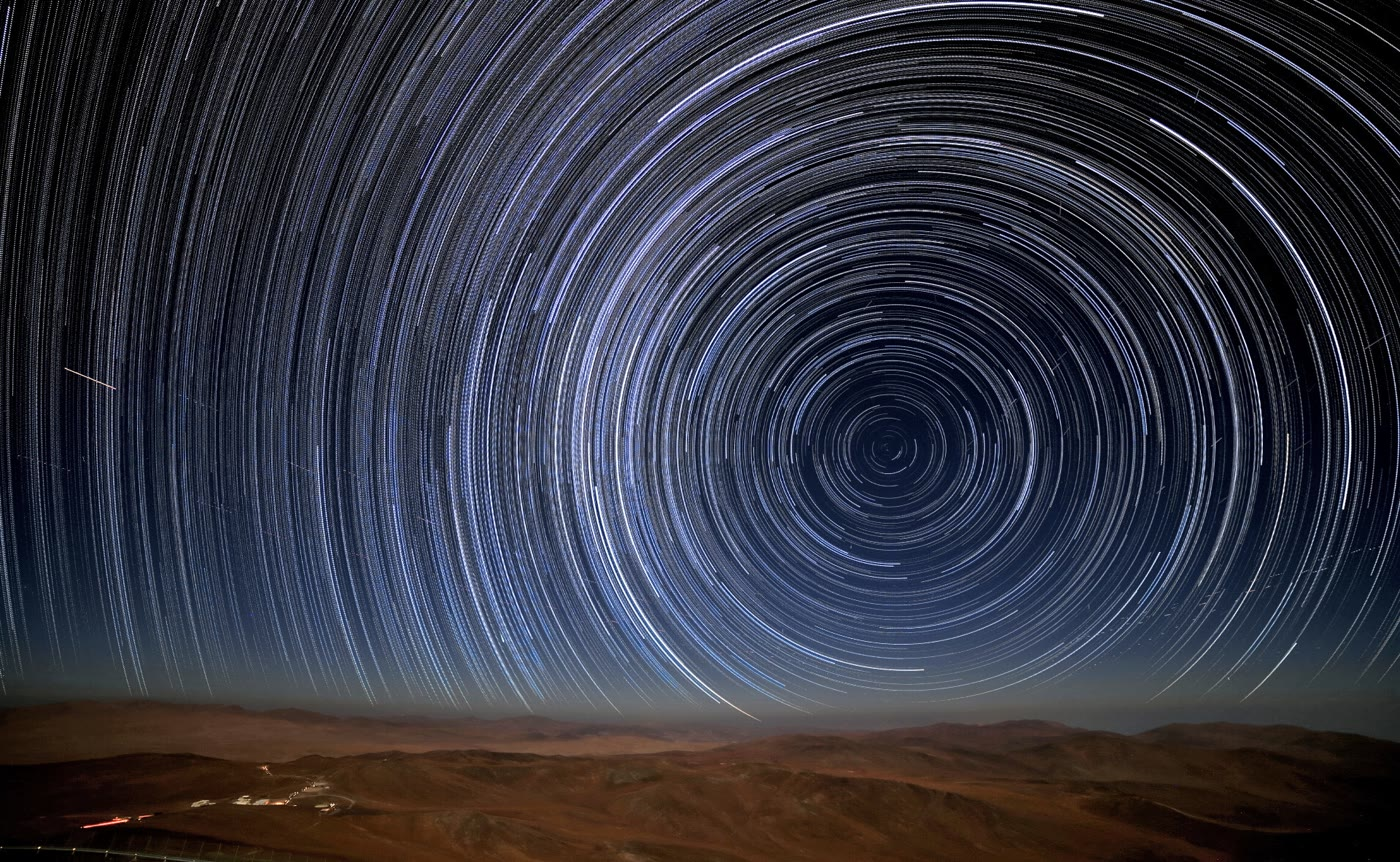
\includegraphics[width=0.8\linewidth]{images/book3/b1-star-trails-paranal.jpg}
% ledger: commons:eso-paranal-star-trails, mpc:paranal

{\small Star trails above the Paranal Observatory, in the Atacama desert, at
\omterm{def:b1:spherical-astronomy:geographic}{latitude} \ang{24.6} S: a long exposure records each star's arc round the
south \omterm{def:b1:spherical-astronomy:celestial-sphere}{celestial pole}, which stands \ang{24.6} above the southern horizon.
Photograph R.~Wesson/ESO, CC BY 4.0.}
\end{omfigure}

\section{Sidereal time and solar time}

\begin{definition}[The ecliptic]\label{def:b1:spherical-astronomy:ecliptic}
The \emph{ecliptic}\index{ecliptic} is the \omterm{def:b1:spherical-astronomy:spherical-triangle}{great circle} of the \omterm{def:b1:spherical-astronomy:celestial-sphere}{celestial
sphere} along which the Sun appears to move in a year, the trace of the plane
of the Earth's orbit. It is inclined to the \omterm{def:b1:spherical-astronomy:celestial-sphere}{celestial equator} by the
\emph{obliquity of the ecliptic}\index{obliquity of the ecliptic}
$\varepsilon$, the tilt of the Earth's axis to its orbit. The ecliptic
crosses the equator at two points; the \emph{vernal equinox
point}\index{vernal equinox point} $\gamma$ is the one where the Sun crosses
the equator northward, in March. The Sun's ecliptic \omterm{def:b1:spherical-astronomy:geographic}{longitude} $\lambda_\odot$
is its angle along the ecliptic from $\gamma$, counted eastward.
\end{definition}

% ledger: earth:obliquity (23.44)
The obliquity is today $\varepsilon = \ang{23.44}$.

\begin{definition}[Sidereal time]\label{def:b1:spherical-astronomy:sidereal-time}
The local \emph{sidereal time}\index{sidereal time} is the \omterm{def:b1:spherical-astronomy:equatorial}{hour angle} of the
\omterm{def:b1:spherical-astronomy:ecliptic}{vernal equinox point} $\gamma$. A sidereal day is the interval between two
passages of $\gamma$ across the meridian.
\end{definition}

Since \omterm{def:b1:spherical-astronomy:equatorial}{right ascension} is counted eastward from $\gamma$ and \omterm{def:b1:spherical-astronomy:equatorial}{hour angle}
westward from the meridian, for every star
\[
  H = \mathrm{LST} - \alpha ,
\]
where LST is the local \omterm{def:b1:spherical-astronomy:sidereal-time}{sidereal time}: a star crosses the meridian when the
\omterm{def:b1:spherical-astronomy:sidereal-time}{sidereal time} equals its \omterm{def:b1:spherical-astronomy:equatorial}{right ascension}. An observatory clock showing
\omterm{def:b1:spherical-astronomy:sidereal-time}{sidereal time} tells at a glance which part of the sky is overhead.

\begin{proposition}[Sidereal and solar days]\label{prop:b1:spherical-astronomy:sidereal-day}
In one \omterm{def:b1:spherical-astronomy:tropical-year}{tropical year} of $N$ mean solar days, the Earth turns $N + 1$ times
relative to the stars. Hence the sidereal day lasts
\[
  \frac{N}{N + 1}\times\qty{24}{h},
\]
and with $N = 365.2422$ this is \qty{23}{h}~\qty{56}{min}~\qty{4.09}{s}: a
star crosses the meridian \qty{3}{min}~\qty{56}{s} of \omterm{def:b1:spherical-astronomy:solar-time}{mean solar time} earlier
each day.
\end{proposition}

\begin{proof}
% ledger: usno:tropical-year, earth:Trot (23.9345 h)
Count turns relative to the Sun and relative to the stars over one year. The
Sun moves once round the \omterm{def:b1:spherical-astronomy:ecliptic}{ecliptic} eastward in a year, in the direction of the
Earth's rotation. Relative to the Sun the Earth therefore makes one turn
fewer than relative to the stars: $N$ solar days and $N + 1$ sidereal days
fill the same year. The sidereal day is $N/(N+1)$ of a solar day, that is
$\qty{86400}{s}\times 365.2422/366.2422 = \qty{86164.09}{s}$; the difference
is $\qty{235.9}{s}$. This agrees with the Earth's measured rotation period
relative to the stars, \qty{23.9345}{h}.
\end{proof}

\begin{definition}[Solar time]\label{def:b1:spherical-astronomy:solar-time}
\emph{Apparent solar time}\index{apparent solar time} is the \omterm{def:b1:spherical-astronomy:equatorial}{hour angle} of
the Sun plus 12 hours: a sundial shows it, and it is noon when the Sun
crosses the meridian. \emph{Mean solar time}\index{mean solar time} is the
\omterm{def:b1:spherical-astronomy:equatorial}{hour angle}, plus 12 hours, of a fictitious mean Sun that moves along the
\omterm{def:b1:spherical-astronomy:celestial-sphere}{celestial equator} at a uniform rate, completing a turn in a \omterm{def:b1:spherical-astronomy:tropical-year}{tropical year}.
Their difference, apparent minus mean, is the \emph{equation of
time}\index{equation of time}.
\end{definition}

The true Sun runs ahead of and behind the mean Sun for two reasons. The
Earth moves faster near perihelion, in early January, than near aphelion, so
the Sun's progress along the \omterm{def:b1:spherical-astronomy:ecliptic}{ecliptic} is uneven (Kepler's second law); and
the Sun moves along the \omterm{def:b1:spherical-astronomy:ecliptic}{ecliptic}, which is inclined to the equator, so that
even a uniform motion along the \omterm{def:b1:spherical-astronomy:ecliptic}{ecliptic} projects onto the equator --- which is
what the \omterm{def:b1:spherical-astronomy:equatorial}{hour angle} measures --- unevenly, faster near the solstices than near
the equinoxes. Civil clocks keep \omterm{def:b1:spherical-astronomy:solar-time}{mean solar time} on a reference meridian of
their time zone; the local mean time at \omterm{def:b1:spherical-astronomy:geographic}{longitude} $\lambda$ is ahead of the
time at Greenwich by $\lambda/\ang{15}$ hours.

\begin{omfigure}
\begin{tikzpicture}
\begin{axis}[omrecord, width=0.9\linewidth, height=5.2cm, xmin=0, xmax=365,
  xtick={0,31,59,90,120,151,181,212,243,273,304,334,365},
  xticklabels={J,F,M,A,M,J,J,A,S,O,N,D,},
  ylabel={equation of time (min)}, ymin=-20, ymax=21,
  tick label style={font=\scriptsize}, label style={font=\small}]
\addplot[black!50, line width=0.4pt] coordinates {(0,0) (365,0)};
\addplot[omDef, line width=1.1pt] table[x=day, y=eot_min] {figdata/out/bachelor-1-day_length-eot.dat};
\node[font=\scriptsize, above, fill=white, inner sep=1pt] at (axis cs:306,16.6) {$+16.4$};
\node[font=\scriptsize, below, fill=white, inner sep=1pt] at (axis cs:41,-14.4) {$-14.2$};
\end{axis}
\end{tikzpicture}

{\small The \omterm{def:b1:spherical-astronomy:solar-time}{equation of time} through the year (apparent minus \omterm{def:b1:spherical-astronomy:solar-time}{mean solar
time}): a sundial is up to \qty{16.4}{min} fast in early November and
\qty{14.2}{min} slow in mid-February. Computed from a Kepler orbit with the
eccentricity 0.0167, the obliquity \ang{23.44}, the \omterm{def:b1:spherical-astronomy:geographic}{longitude} of perihelion
and the date of the 2026 March equinox.}
% ledger: earth:ecc, earth:obliquity, nasa:earth-perihelion-longitude, usno:seasons-2026
\end{omfigure}

\section{Rising, setting and the Sun}

\begin{proposition}[Rising and setting]\label{prop:b1:spherical-astronomy:rising}
At \omterm{def:b1:spherical-astronomy:geographic}{latitude} $\varphi$, a star of \omterm{def:b1:spherical-astronomy:equatorial}{declination} $\delta$ that rises and sets
crosses the horizon at the \omterm{def:b1:spherical-astronomy:equatorial}{hour angles} $\pm H_0$ with
\[
  \cos H_0 = -\tan\varphi\tan\delta ,
\]
at the \omterm{def:b1:spherical-astronomy:horizontal}{azimuth} $\mathrm{A}_0$ with $\cos\mathrm{A}_0 = \sin\delta/\cos\varphi$
(rising; it sets at $\ang{360} - \mathrm{A}_0$). It stays above the horizon
for $2H_0$, converted to hours at \ang{15} per hour.
\end{proposition}

\begin{proof}
On the horizon $h = 0$, and \cref{prop:b1:spherical-astronomy:transform}
gives $0 = \sin\varphi\sin\delta + \cos\varphi\cos\delta\cos H_0$, and
$\cos\mathrm{A}_0 = \sin\delta/\cos\varphi$. The \omterm{def:b1:spherical-astronomy:equatorial}{hour angle} grows uniformly,
by \ang{15} per hour, from $-H_0$ at rising to $+H_0$ at setting.
\end{proof}

For the Sun this gives the length of the day, if the Sun is treated as a
point and the bending of light by the air is ignored (both add a few minutes
of daylight). At the equinoxes $\delta = 0$, $H_0 = \ang{90}$: day and night
last twelve hours everywhere, and the Sun rises due east.

\begin{omfigure}
\begin{tikzpicture}
\begin{axis}[omrecord, width=0.85\linewidth, height=5.6cm, xmin=40, xmax=320, ymin=0, ymax=75,
  xtick={45,90,135,180,225,270,315}, xticklabels={NE,E,SE,S,SW,W,NW}, ytick={0,15,30,45,60,75},
  xlabel={azimuth}, ylabel={altitude of the Sun ($^\circ$)},
  tick label style={font=\scriptsize}, label style={font=\small}]
\addplot[omThm, line width=1pt] table[x=az_deg, y=alt_deg] {figdata/out/bachelor-1-sun_paths-june.dat};
\addplot[black, line width=1pt] table[x=az_deg, y=alt_deg] {figdata/out/bachelor-1-sun_paths-equinox.dat};
\addplot[omDef, line width=1pt] table[x=az_deg, y=alt_deg] {figdata/out/bachelor-1-sun_paths-december.dat};
\begin{scope}[font=\scriptsize, fill=white, fill opacity=0.8, text opacity=1, inner sep=1pt]
  \node[omThm, above, fill=white] at (axis cs:180,68.4) {June solstice, $\ang{68.4}$};
  \node[above, fill=white] at (axis cs:180,45) {equinoxes, $\ang{45}$};
  \node[omDef, above, fill=white] at (axis cs:180,21.6) {December solstice, $\ang{21.6}$};
\end{scope}
\end{axis}
\end{tikzpicture}

{\small The Sun's path across the sky at \omterm{def:b1:spherical-astronomy:geographic}{latitude} \ang{45} N at the June
solstice (red), the equinoxes (black) and the December solstice (blue), with
the noon \omterm{def:b1:spherical-astronomy:horizontal}{altitudes} $\ang{90} - \varphi + \delta_\odot$. At the equinoxes the
Sun rises due east and sets due west; in June it rises in the north-east.}
\end{omfigure}

\begin{proposition}[The Sun's declination]\label{prop:b1:spherical-astronomy:sun-declination}
When the Sun is at the \omterm{def:b1:spherical-astronomy:ecliptic}{ecliptic} \omterm{def:b1:spherical-astronomy:geographic}{longitude} $\lambda_\odot$, its \omterm{def:b1:spherical-astronomy:equatorial}{declination} and
\omterm{def:b1:spherical-astronomy:equatorial}{right ascension} satisfy
\[
  \sin\delta_\odot = \sin\varepsilon\sin\lambda_\odot, \qquad
  \tan\alpha_\odot = \cos\varepsilon\tan\lambda_\odot .
\]
\end{proposition}

\begin{proof}
Take axes with $x$ toward $\gamma$ and $z$ toward the north \omterm{def:b1:spherical-astronomy:celestial-sphere}{celestial pole}.
In axes $x$, $y'$, $z'$ attached to the \omterm{def:b1:spherical-astronomy:ecliptic}{ecliptic}, with $z'$ toward its pole,
the Sun's direction is $(\cos\lambda_\odot, \sin\lambda_\odot, 0)$. The
\omterm{def:b1:spherical-astronomy:ecliptic}{ecliptic} axes are those of the equator turned by the angle $\varepsilon$ about
$x$, so in equatorial axes the Sun's direction is
$(\cos\lambda_\odot,\ \sin\lambda_\odot\cos\varepsilon,\
\sin\lambda_\odot\sin\varepsilon)$. Its $z$ component is $\sin\delta_\odot$;
the ratio of its $y$ and $x$ components is $\tan\alpha_\odot$.
\end{proof}

\begin{omfigure}
\begin{tikzpicture}
\begin{axis}[omrecord, width=0.9\linewidth, height=6cm, xmin=0, xmax=365, ymin=0, ymax=24,
  xtick={0,31,59,90,120,151,181,212,243,273,304,334,365},
  xticklabels={J,F,M,A,M,J,J,A,S,O,N,D,}, ytick={0,6,12,18,24},
  ylabel={day length (h)}, tick label style={font=\scriptsize}, label style={font=\small},
  legend style={font=\scriptsize, at={(0.5,1.02)}, anchor=south, draw=none}, legend columns=5,
  legend cell align=left]
\addplot[black, line width=0.9pt] table[x=day, y=lat0] {figdata/out/bachelor-1-day_length-lengths.dat};
\addplot[omDef, line width=0.9pt] table[x=day, y=lat30] {figdata/out/bachelor-1-day_length-lengths.dat};
\addplot[omThm, line width=0.9pt] table[x=day, y=lat45] {figdata/out/bachelor-1-day_length-lengths.dat};
\addplot[omField, line width=0.9pt] table[x=day, y=lat60] {figdata/out/bachelor-1-day_length-lengths.dat};
\addplot[black, line width=0.9pt, densely dashed] table[x=day, y=lat70] {figdata/out/bachelor-1-day_length-lengths.dat};
\legend{\ang{0}, \ang{30} N, \ang{45} N, \ang{60} N, \ang{70} N}
\end{axis}
\end{tikzpicture}

{\small Length of the day (Sun's centre above the geometric horizon) through
the year at five northern \omterm{def:b1:spherical-astronomy:geographic}{latitudes}, from
\cref{prop:b1:spherical-astronomy:rising,prop:b1:spherical-astronomy:sun-declination}.
At \ang{70} N the Sun stays up for weeks around the June solstice and stays
down around the December solstice. In the southern hemisphere the curves are
shifted by half a year.}
\end{omfigure}

\begin{definition}[Insolation]\label{def:b1:spherical-astronomy:insolation}
The \emph{insolation}\index{insolation} at a place and an instant is the
power of sunlight received per unit area of a horizontal surface at the top
of the atmosphere. With $S_0$ the solar irradiance at the mean distance $a$
of the Sun, $r$ the actual distance and $\theta_z$ the Sun's \omterm{def:b1:spherical-astronomy:celestial-sphere}{zenith} distance,
\[
  I = S_0\left(\frac{a}{r}\right)^{2}\cos\theta_z = S_0\left(\frac{a}{r}\right)^{2}\sin h_\odot
  \quad (h_\odot > 0), \qquad I = 0 \text{ at night}.
\]
\end{definition}

% ledger: earth:TSI (1361 W/m2), earth:peri, earth:aph, earth:a
The factor $(a/r)^2$ is the inverse-square law for light (the physics books);
the factor $\cos\theta_z$ appears because a beam of cross-section one square
metre spreads over $1/\cos\theta_z$ square metres of horizontal ground. With
$S_0 = \qty{1361}{W.m^{-2}}$ and a Sun--Earth distance between
\qty{147.1e6}{km} at perihelion and \qty{152.1e6}{km} at aphelion, the factor
$(a/r)^2$ varies by $\pm\qty{3.4}{\percent}$ in the year. The tilt of the axis
does much more: it changes both the noon \omterm{def:b1:spherical-astronomy:horizontal}{altitude} and the day length, and
these two together make the seasons. The daily and yearly sums of the
\omterm{def:b1:spherical-astronomy:insolation}{insolation}, which drive the climate, are computed in
\cref{ch:b1:radiation-heat-transport}.


\section{Calendars}

\begin{definition}[Tropical year]\label{def:b1:spherical-astronomy:tropical-year}
The \emph{tropical year}\index{tropical year} is the mean interval between
two passages of the Sun through the \omterm{def:b1:spherical-astronomy:ecliptic}{vernal equinox point}. It governs the
seasons; it lasts 365.2422 mean solar days.
\end{definition}

% ledger: usno:tropical-year, earth:Psid (365.256 d)
The \omterm{def:b1:spherical-astronomy:tropical-year}{tropical year} is about twenty minutes shorter than the sidereal year, the
time the Earth takes to come back to the same place among the stars
(365.256 days), because the Earth's axis slowly turns --- it precesses --- and
carries the equinox point backward along the \omterm{def:b1:spherical-astronomy:ecliptic}{ecliptic} (the Year 2 volume).
A calendar must fit a whole number of days to the \omterm{def:b1:spherical-astronomy:tropical-year}{tropical year}, so that the
seasons come back on the same dates.

\begin{proposition}[The Gregorian year]\label{prop:b1:spherical-astronomy:gregorian}
In the Gregorian calendar, a year is a leap year of 366 days if its number is
divisible by 4, except the century years, which are leap years only if
divisible by 400. Its mean year is
\[
  365 + \frac14 - \frac1{100} + \frac1{400} = \num{365.2425}\text{ days},
\]
and it drifts against the seasons by one day in about 3300 years.
\end{proposition}

\begin{proof}
% ledger: usno:leap-rule, usno:tropical-year
In 400 years there are 100 years divisible by 4; among them are four
century years, of which three are not divisible by 400. So there are 97 leap
years and $400\times 365 + 97 = 146\,097$ days,
that is 365.2425 days a year. Against a \omterm{def:b1:spherical-astronomy:tropical-year}{tropical year} of 365.2422 days the
excess is 0.0003 days a year: one day in $1/0.0003 \approx 3300$ years.
\end{proof}

\begin{history}[The reform of 1582]
% ledger: usno:gregorian-1582
The Julian calendar, inherited from Rome, added a leap day every fourth
year: its year of 365.25 days is longer than the \omterm{def:b1:spherical-astronomy:tropical-year}{tropical year} by 0.0078
days, a day in 128 years. Over the centuries the date of the vernal equinox
drifted away from 21 March, the date on which the reckoning of Easter relied.
In 1582 Pope Gregory~XIII introduced the calendar that bears his name, which
dropped the accumulated days at once and replaced the Julian rule by the rule
of \cref{prop:b1:spherical-astronomy:gregorian}. It has become the
internationally accepted civil calendar.
\end{history}

\begin{inthefield}[Finding a position from the stars]
Before satellite positioning, navigators at sea found their \omterm{def:b1:spherical-astronomy:geographic}{latitude} and
\omterm{def:b1:spherical-astronomy:geographic}{longitude} from the sky. With a sextant they measured the \omterm{def:b1:spherical-astronomy:horizontal}{altitude} of the Sun
at noon, or of two or three stars at dusk, and read the time on a chronometer
kept on the time of the Greenwich meridian. Each \omterm{def:b1:spherical-astronomy:horizontal}{altitude}, with the star's
\omterm{def:b1:spherical-astronomy:equatorial}{declination} and its \omterm{def:b1:spherical-astronomy:equatorial}{hour angle} at Greenwich from an almanac, gives a \omterm{def:b1:spherical-astronomy:spherical-triangle}{small
circle} on the Earth on which the ship lies: the circle of points where the
star is at that \omterm{def:b1:spherical-astronomy:horizontal}{altitude}. Two or three such circles cross at the ship's
position --- spherical trigonometry solved at sea every day. The noon
\omterm{def:b1:spherical-astronomy:horizontal}{altitude} of the Sun alone gives the \omterm{def:b1:spherical-astronomy:geographic}{latitude}
(\cref{prop:b1:spherical-astronomy:culmination}); the clock time of local
noon gives the \omterm{def:b1:spherical-astronomy:geographic}{longitude}, at four minutes of time per degree.
\begin{center}
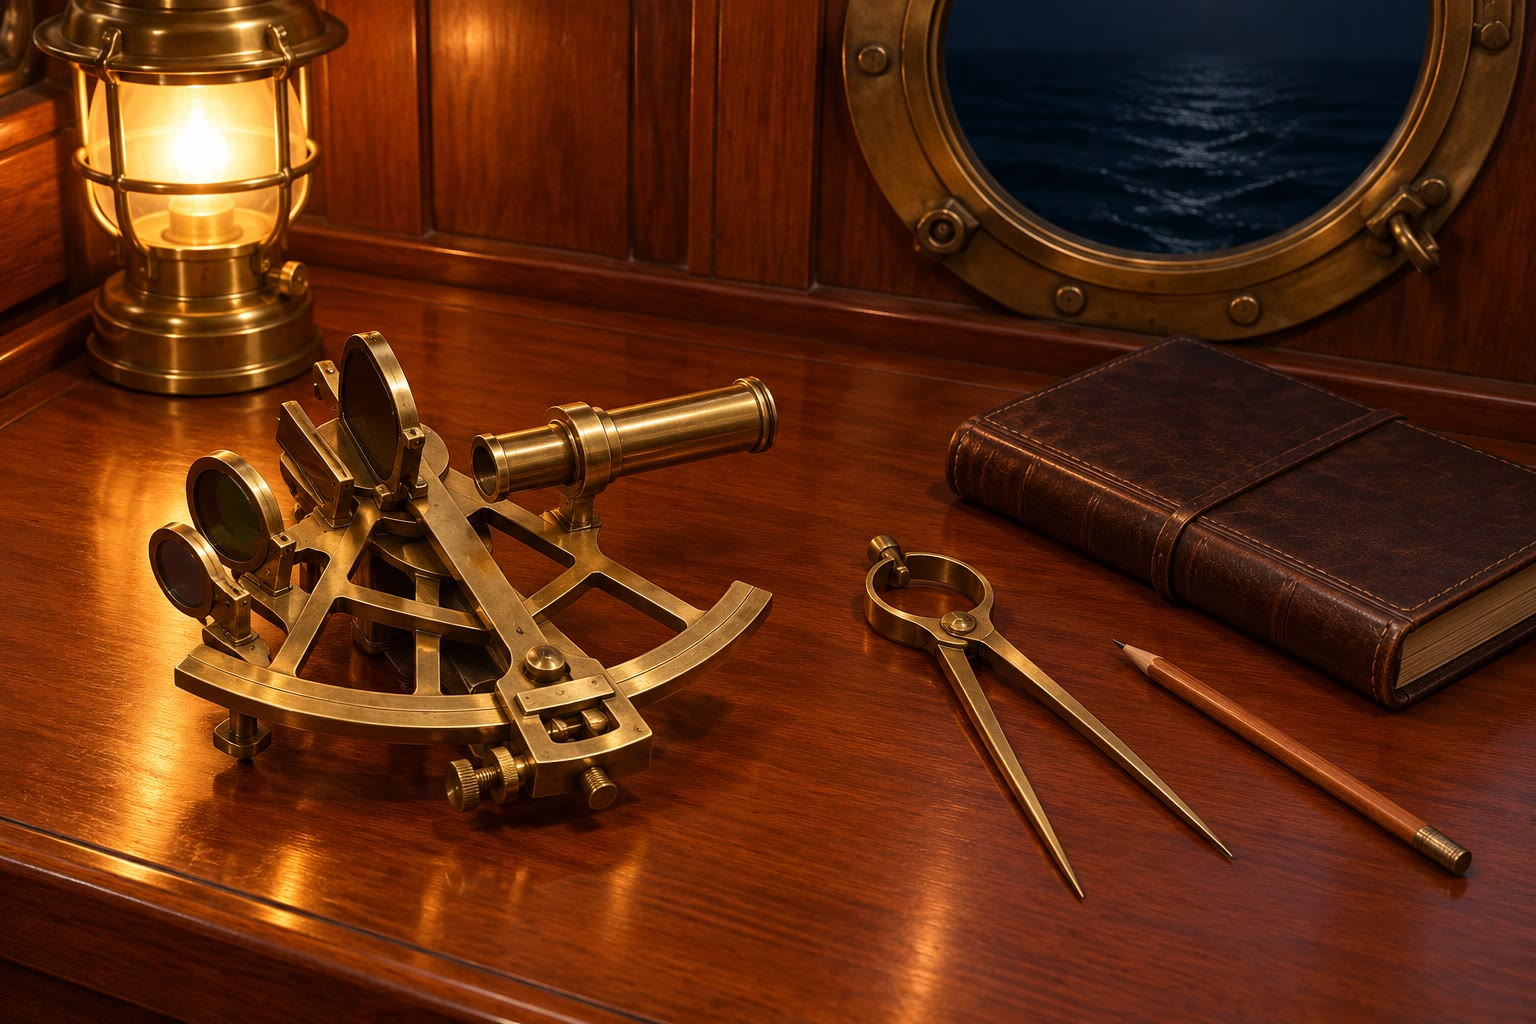
\includegraphics[width=0.55\linewidth]{images/book3/ai/b1-sextant.jpg}
\end{center}
\end{inthefield}

\section{Exercises}

\begin{exercise}[$\star$]\label{exo:b1:spherical-astronomy:1}
An observer is at \omterm{def:b1:spherical-astronomy:geographic}{latitude} \ang{52} N. At what \omterm{def:b1:spherical-astronomy:horizontal}{altitude} does the north
\omterm{def:b1:spherical-astronomy:celestial-sphere}{celestial pole} stand? Which stars, by their \omterm{def:b1:spherical-astronomy:equatorial}{declination}, never set there, and
which never rise?
\end{exercise}

\begin{exercise}[$\star$]\label{exo:b1:spherical-astronomy:2}
Convert a \omterm{def:b1:spherical-astronomy:equatorial}{right ascension} of \qty{6}{h}~\qty{45}{min} into degrees. At a
local \omterm{def:b1:spherical-astronomy:sidereal-time}{sidereal time} of \qty{10}{h}~\qty{0}{min}, what is the \omterm{def:b1:spherical-astronomy:equatorial}{hour angle} of a
star of that \omterm{def:b1:spherical-astronomy:equatorial}{right ascension}? Is the star east or west of the meridian?
\end{exercise}

\begin{exercise}[$\star$]\label{exo:b1:spherical-astronomy:3}
At \omterm{def:b1:spherical-astronomy:geographic}{latitude} \ang{40} N, compute the \omterm{def:b1:spherical-astronomy:horizontal}{altitude} of the Sun at noon at the two
solstices and at the equinoxes ($\varepsilon = \ang{23.44}$).
\end{exercise}

\begin{exercise}[$\star$]\label{exo:b1:spherical-astronomy:4}
Was 1900 a leap year? Was 2000? Will 2100 be? By how many days per century
does the Julian calendar drift against a \omterm{def:b1:spherical-astronomy:tropical-year}{tropical year} of 365.2422 days, and
by how many does the Gregorian calendar?
\end{exercise}

\begin{exercise}[$\star\star$]\label{exo:b1:spherical-astronomy:5}
Two points lie at \omterm{def:b1:spherical-astronomy:geographic}{latitude} \ang{45} N, at \omterm{def:b1:spherical-astronomy:geographic}{longitudes} \ang{0} and
\ang{90} E. Compute the great-circle distance between them
($R = \qty{6371}{km}$) and the distance along their parallel. Which is
shorter, and by how much?
\end{exercise}

\begin{exercise}[$\star\star$]\label{exo:b1:spherical-astronomy:6}
At \omterm{def:b1:spherical-astronomy:geographic}{latitude} \ang{48} N, a star of \omterm{def:b1:spherical-astronomy:equatorial}{declination} \ang{20} has the \omterm{def:b1:spherical-astronomy:equatorial}{hour angle}
\ang{30}. Compute its \omterm{def:b1:spherical-astronomy:horizontal}{altitude} and its \omterm{def:b1:spherical-astronomy:horizontal}{azimuth}. In which direction should the
observer look?
\end{exercise}

\begin{exercise}[$\star\star$]\label{exo:b1:spherical-astronomy:7}
Compute the length of the day at \omterm{def:b1:spherical-astronomy:geographic}{latitude} \ang{60} N at the June solstice,
the Sun being treated as a point on a geometric horizon. Check your answer on
the day-length figure.
\end{exercise}

\begin{exercise}[$\star\star$]\label{exo:b1:spherical-astronomy:8}
A star crosses the meridian tonight at 22:00 local mean time. At what time
will it cross the meridian in 30 days? In how many days will it cross at
noon, invisible in daylight?
\end{exercise}

\begin{exercise}[$\star\star$]\label{exo:b1:spherical-astronomy:9}
Compute the \omterm{def:b1:spherical-astronomy:insolation}{insolation} at the top of the atmosphere at noon at \omterm{def:b1:spherical-astronomy:geographic}{latitude}
\ang{45} N (a) at an equinox, taking $r = a$; (b) at the June solstice,
taking for $r$ the aphelion distance. Data: $S_0 = \qty{1361}{W.m^{-2}}$,
$a = \qty{149.598e6}{km}$, aphelion \qty{152.100e6}{km}.
\end{exercise}

\begin{exercise}[$\star\star\star$]\label{exo:b1:spherical-astronomy:10}
Using \cref{prop:b1:spherical-astronomy:sun-declination}, compute the
\omterm{def:b1:spherical-astronomy:equatorial}{declination} and the \omterm{def:b1:spherical-astronomy:equatorial}{right ascension} of the Sun when its \omterm{def:b1:spherical-astronomy:ecliptic}{ecliptic} \omterm{def:b1:spherical-astronomy:geographic}{longitude}
is \ang{60}. By how many degrees does the \omterm{def:b1:spherical-astronomy:equatorial}{right ascension} lag behind the
\omterm{def:b1:spherical-astronomy:geographic}{longitude}? Explain with this result why the inclination of the \omterm{def:b1:spherical-astronomy:ecliptic}{ecliptic}
contributes to the \omterm{def:b1:spherical-astronomy:solar-time}{equation of time}.
\end{exercise}

\begin{exercise}[$\star\star\star$]\label{exo:b1:spherical-astronomy:11}
Show that at the June solstice the Sun rises at the \omterm{def:b1:spherical-astronomy:horizontal}{azimuth} $\mathrm{A}_0$
with $\cos\mathrm{A}_0 = \sin\varepsilon/\cos\varphi$. At what \omterm{def:b1:spherical-astronomy:geographic}{latitude} does
it rise exactly in the north-east? What happens to the formula at \omterm{def:b1:spherical-astronomy:geographic}{latitudes}
above $\ang{90} - \varepsilon$?
\end{exercise}

\begin{exercise}[$\star\star\star$]\label{exo:b1:spherical-astronomy:12}
A lune is the part of a sphere between two half \omterm{def:b1:spherical-astronomy:spherical-triangle}{great circles} joining two
opposite points, at the angle $\theta$ to each other. (a) Show that its area
is $2\theta R^2$. (b) Each side of a \omterm{def:b1:spherical-astronomy:spherical-triangle}{spherical triangle} $ABC$, prolonged into
a full \omterm{def:b1:spherical-astronomy:spherical-triangle}{great circle}, gives with the others three pairs of opposite lunes of
angles $A$, $B$, $C$ that cover the sphere, the triangle and its opposite
being covered three times. Deduce Girard's theorem: the triangle's area is
$R^2(A + B + C - \pi)$. (c) Apply it to the triangle with three right angles,
and to the triangle drawn in this chapter (angles \ang{89.9}, \ang{64.9},
\ang{67.4}).
\end{exercise}

\section{Problem: A night at a mountain observatory}

\begin{problem}[{Weekend problem --- where the Paranal Observatory stands, what
its sky shows, and how long its longest night lasts}]
\label{pb:b1:spherical-astronomy:1}
% ledger: mpc:paranal, mpc:greenwich, simbad:sirius, simbad:canopus, usno:seasons-2026, earth:obliquity, usno:tropical-year
% numbers computed in the scratch calculator calc/ch01.py from the rounded data
The Paranal Observatory stands in the Atacama desert at \omterm{def:b1:spherical-astronomy:geographic}{latitude}
\ang{24.63} S, \omterm{def:b1:spherical-astronomy:geographic}{longitude} \ang{70.40} W. The Royal Observatory at Greenwich,
through which \omterm{def:b1:spherical-astronomy:geographic}{longitudes} are counted, is at \ang{51.48} N, \ang{0.00}. Two
bright stars of the southern sky have the coordinates
\begin{center}
\small
\begin{tabular}{lcc}
\hline
star & \omterm{def:b1:spherical-astronomy:equatorial}{right ascension} & \omterm{def:b1:spherical-astronomy:equatorial}{declination} \\
\hline
Sirius & \qty{6}{h}~\qty{45}{min}~\qty{9}{s} & \ang{-16.72} \\
Canopus & \qty{6}{h}~\qty{23}{min}~\qty{57}{s} & \ang{-52.70} \\
\hline
\end{tabular}
\end{center}
Take $R = \qty{6371}{km}$, $\varepsilon = \ang{23.44}$, a \omterm{def:b1:spherical-astronomy:tropical-year}{tropical year} of
365.2422 days, and treat the Sun as a point on a geometric horizon.

\medskip
\noindent\textbf{Part I --- Paranal on the globe.}
\begin{enumerate}
  \item Give the colatitudes of Paranal and Greenwich, and their difference
        of \omterm{def:b1:spherical-astronomy:geographic}{longitude}.
  \item Write the cosine rule for the triangle North Pole--Paranal--Greenwich
        and compute the cosine of the angular distance $\Delta$ between the
        two observatories.
  \item Deduce $\Delta$ in degrees and the great-circle distance in
        kilometres.
  \item Compute the initial heading from Paranal toward Greenwich
        (\cref{met:b1:spherical-astronomy:great-circle}).
  \item Check the heading with the sine rule.
  \item Would an aircraft keeping this heading all the way reach Greenwich?
        Explain.
\end{enumerate}

\medskip
\noindent\textbf{Part II --- The sky of Paranal.}
\begin{enumerate}[resume]
  \item At what \omterm{def:b1:spherical-astronomy:horizontal}{altitude} does the south \omterm{def:b1:spherical-astronomy:celestial-sphere}{celestial pole} stand above the
        southern horizon of Paranal?
  \item At what \omterm{def:b1:spherical-astronomy:horizontal}{altitude} does Sirius cross the meridian, and on which side of
        the \omterm{def:b1:spherical-astronomy:celestial-sphere}{zenith}?
  \item Below which \omterm{def:b1:spherical-astronomy:equatorial}{declination} is a star circumpolar at Paranal? Is Canopus
        circumpolar?
  \item What is the highest \omterm{def:b1:spherical-astronomy:horizontal}{altitude} Canopus reaches?
  \item Compute the \omterm{def:b1:spherical-astronomy:equatorial}{hour angle} at which Sirius rises, and how long it stays
        above the horizon, in sidereal hours.
  \item At what \omterm{def:b1:spherical-astronomy:horizontal}{azimuth} does Sirius rise?
\end{enumerate}

\medskip
\noindent\textbf{Part III --- Clocks.}
\begin{enumerate}[resume]
  \item What is the local \omterm{def:b1:spherical-astronomy:sidereal-time}{sidereal time} when Sirius crosses the meridian?
  \item Compute the length of the sidereal day, and by how many minutes a
        star's meridian passage moves earlier each night.
  \item Take the local \omterm{def:b1:spherical-astronomy:sidereal-time}{sidereal time} at local mean midnight to be
        \qty{12}{h} on the March equinox (20 March 2026), when the Sun is near
        the \omterm{def:b1:spherical-astronomy:ecliptic}{vernal equinox point}; it then gains $24/365.2422$ hours a day.
        How many days after the equinox does Sirius cross the meridian at
        local mean midnight? On what date?
  \item On that night, by how much does local mean time at Paranal differ
        from the time at Greenwich?
  \item The \omterm{def:b1:spherical-astronomy:solar-time}{equation of time} is then about \qty{-3}{min}. What time does a
        sundial at the observatory show (\omterm{def:b1:spherical-astronomy:solar-time}{apparent solar time}) when Sirius
        crosses the meridian?
  \item How much earlier does it cross one week later?
\end{enumerate}

\medskip
\noindent\textbf{Part IV --- The longest night.}
\begin{enumerate}[resume]
  \item What is the Sun's \omterm{def:b1:spherical-astronomy:equatorial}{declination} at each solstice?
  \item Compute the \omterm{def:b1:spherical-astronomy:horizontal}{altitude} of the Sun at noon at Paranal at the June and
        December solstices. On which side of the \omterm{def:b1:spherical-astronomy:celestial-sphere}{zenith} is it in December?
  \item At the December solstice the Sun--Earth distance is 0.9837 times the
        mean distance. Compute the \omterm{def:b1:spherical-astronomy:insolation}{insolation} at noon at the top of the
        atmosphere above Paranal ($S_0 = \qty{1361}{W.m^{-2}}$).
  \item At which solstice is the night longest at Paranal? Compute the \omterm{def:b1:spherical-astronomy:equatorial}{hour
        angle} of sunset on that date.
  \item At what \omterm{def:b1:spherical-astronomy:horizontal}{azimuth} does the Sun rise on that date?
  \item Deduce the length of the longest night of the year at Paranal, in
        hours and minutes.
\end{enumerate}
\end{problem}
